\subsection{Action Frame Generation}
%This subsection evaluates our ability to automatically infer fuzzy clusters of verbs.
We apply ActionNet(PB), which covers most of the verbs
and arguments, to action frame generation problem.
We cluster the verbs into fuzzy clusters and assign each
fuzzy cluster an action frame.
%For example, ``buy'' and ``sell'' have the similar usage
%and meaning of ``business deal''.
%In our action concept lexicon, concepts for their objects are almost the same, they are ``product'', ``service'', ``application'' and ``source''. Therefore, regarding our action concepts as a semantic feature, it is able to process verb clustering task.
Since verbs with similar semantics have similar action concepts in our lexicon,
we cluster the verbs by their action concepts.

With concepts extracted from the dataset, we draw a concept histogram for
each verb, which represents the semantic information.
We use the \emph{Vector Space Model} (VSM) to represent the context.
We define a probability distribution score for each dimension
by the IsA relation between the concept and the argument instance as:
$$
Prob(c,v)=\frac{\sum_{e\in E_c\cap A_v}{\frac{freq(e,v)}{|\{c'|c'\in C_k,
e\in E_{c'}\}|}}}{\sum_{c_i\in C_k}{\sum_{e\in E_{c_i}\cap A_v}{\frac{freq(e,v)}{|\{c'|c'\in C_k, e\in E_{c'}\}|}}}},
$$
where $E_c$ is the set of entities covered by concept $c$ in Probase, $A_v$ represents the set of argument instances
for a verb $v$, $freq(e,v)$ is the frequency of the argument $e$ along with verb $v$ in dataset and $C_k$ is the set of concepts for $v$.
%In this experiment, the number of concepts we use is $k=10$.

In order to capture the polysemy of verbs, we apply
a Fuzzy C-means clustering method\cite{dunn73:fuzzycmeans}
that may assign an item
to more than one cluster. We adopt \emph{cosine similarity}
to compute the pairwise similarity of contexts.
The fuzzy clustering process returns for each verb the coefficient
of being in each cluster, namely $Co(v,c)$.
%In order to find the
%strongest signal of a verb belonging to a cluster,
We design
the following condition to determine if a verb $v_i$
belongs to a cluster $c_j$:
$$
Co(v_i,c_j) \geq \mu_{v_i} + 3 \times \sigma_{v_i},
$$
where $\mu_{v_i}$ and $\sigma_{v_i}$ represents the mean and
standard deviation of the coefficients of the verb $v_i$
being in a cluster.
In the case that a verb has no strong signal of
belonging to a cluster, we make the verb itself a cluster.
\tabref{tab:cluster} shows an example of the clustering results.
\begin{table}[th]
\center
\scriptsize
\caption{An example of verb clustering results}
\begin{tabular}{|l|l|}
\hline
ID  &   Verb Cluster \\
\hline \hline
1   &   preach, accept, refuse, negotiate\\
\hline
\multirow{2}{*}{2}
    &   write, ask, read, omit\\
    &   believe, sacrifice, bear, remember\\
\hline
\multirow{2}{*}{3}
    &   change, vary, alter\\
    &   assume, consider\\
\hline
\multirow{2}{*}{4}
    &   open, fill, close, empty \\
    &   clear, form, pave, cover \\
\hline
\end{tabular}
\label{tab:cluster}
\end{table}

%To evaluate the result of verb clustering, we view it as a series of decisions,
%one for each of the $N(N-1)/2$ pairs of $N$ verbs in the collection.
%We assign two verbs to the same cluster if and only if they
%are similar. A true positive (TP) decision assigns two similar verbs
%to the same cluster, a true negative (TN) decision assigns two dissimilar
%verbs to different clusters. There are two types of errors we can commit.
%A false positive (FP) decision assigns two dissimilar verbs to the same cluster.
%A false negative (FN) decision assigns two similar verbs to different clusters.
%We show it in \tabref{evaluate}.
%\begin{table*}[th]
%\small
%\caption{Explanation about TP, TN, FP and FN}
%\begin{tabular}{|l|l|l|}
%\hline
% & Same cluster & Different clusters\\
%\hline
%Same class & TP & FN\\
%\hline
%Different classes & FP & TN\\
%\hline
%\end{tabular}
%\label{evaluate}
%\end{table*}

%Here we use the metric of Rand Index (RI)\cite{1961008} to evaluate the clustering
%result, which measures the percentage of decisions that are correct.
%$$
%RI=\frac{TP+TN}{TP+FP+TN+FN}
%$$

To evaluate the quality of the action frames,
we adopt a subset of Levin's Verb Classes as golden standard data,
in which 2620 verbs are clustered to 261 classes. In Levin's work\cite{1415692}, she classifies
over 3000 English verbs according to shared meaning and behavior.
%Levin starts with
%the hypothesis that a verb's meaning influences its syntactic behavior and develops
%it into a powerful tool for studying the English verb lexicon.
We use the Rand Index (RI)\cite{1961008} as a metric to evaluate
the clustering result, which measures the percentage of correct
assignment of verbs to clusters.

%For comparison against the fuzzy clustering result, we implement the algorithm with
%our action concepts and SP concepts, the result is shown below.
We compare the fuzzy clustering results using action concepts against the results using
SP concepts.
We note that the fuzzy c-means has one parameter $m$, which is used to determine the level of cluster fuzziness.
To examine how the parameter affects the overall performance of the algorithm,
we conduct the experiment by varying $m$.
\figref{fig:cluster} illustrates the RI of clusters against the value of $m$.
We use the number of clusters $C=261$, which is the same as the number of
Levin's Classes.
As shown in the figure, the performance of verb clustering
using action concepts as features is better than using SP concepts.
\begin{figure}[th]
\centering
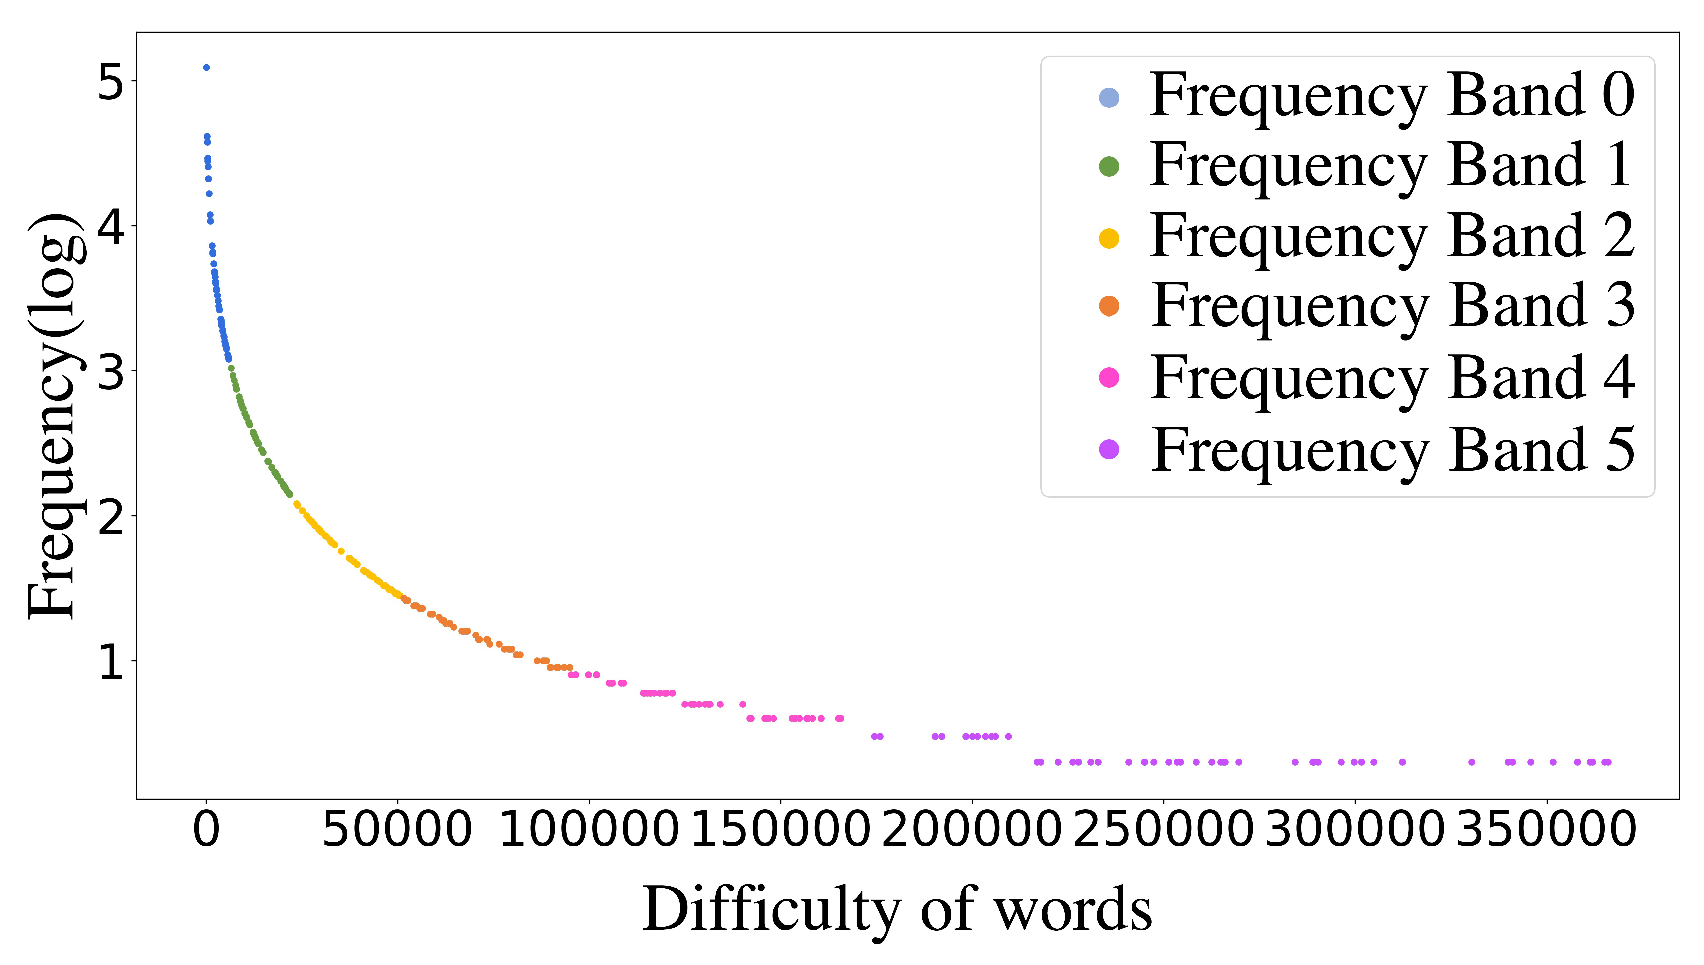
\epsfig{file=figure/cluster.eps,width=.6\columnwidth}
%\vspace*{-5ex}
\caption{RI against fuzzifier $m$}
\label{fig:cluster}
\end{figure}
